% Options for packages loaded elsewhere
\PassOptionsToPackage{unicode}{hyperref}
\PassOptionsToPackage{hyphens}{url}
\PassOptionsToPackage{dvipsnames,svgnames,x11names}{xcolor}
%
\documentclass[
  letterpaper,
  DIV=11,
  numbers=noendperiod]{scrartcl}

\usepackage{amsmath,amssymb}
\usepackage{iftex}
\ifPDFTeX
  \usepackage[T1]{fontenc}
  \usepackage[utf8]{inputenc}
  \usepackage{textcomp} % provide euro and other symbols
\else % if luatex or xetex
  \usepackage{unicode-math}
  \defaultfontfeatures{Scale=MatchLowercase}
  \defaultfontfeatures[\rmfamily]{Ligatures=TeX,Scale=1}
\fi
\usepackage{lmodern}
\ifPDFTeX\else  
    % xetex/luatex font selection
\fi
% Use upquote if available, for straight quotes in verbatim environments
\IfFileExists{upquote.sty}{\usepackage{upquote}}{}
\IfFileExists{microtype.sty}{% use microtype if available
  \usepackage[]{microtype}
  \UseMicrotypeSet[protrusion]{basicmath} % disable protrusion for tt fonts
}{}
\makeatletter
\@ifundefined{KOMAClassName}{% if non-KOMA class
  \IfFileExists{parskip.sty}{%
    \usepackage{parskip}
  }{% else
    \setlength{\parindent}{0pt}
    \setlength{\parskip}{6pt plus 2pt minus 1pt}}
}{% if KOMA class
  \KOMAoptions{parskip=half}}
\makeatother
\usepackage{xcolor}
\setlength{\emergencystretch}{3em} % prevent overfull lines
\setcounter{secnumdepth}{-\maxdimen} % remove section numbering
% Make \paragraph and \subparagraph free-standing
\ifx\paragraph\undefined\else
  \let\oldparagraph\paragraph
  \renewcommand{\paragraph}[1]{\oldparagraph{#1}\mbox{}}
\fi
\ifx\subparagraph\undefined\else
  \let\oldsubparagraph\subparagraph
  \renewcommand{\subparagraph}[1]{\oldsubparagraph{#1}\mbox{}}
\fi

\usepackage{color}
\usepackage{fancyvrb}
\newcommand{\VerbBar}{|}
\newcommand{\VERB}{\Verb[commandchars=\\\{\}]}
\DefineVerbatimEnvironment{Highlighting}{Verbatim}{commandchars=\\\{\}}
% Add ',fontsize=\small' for more characters per line
\usepackage{framed}
\definecolor{shadecolor}{RGB}{241,243,245}
\newenvironment{Shaded}{\begin{snugshade}}{\end{snugshade}}
\newcommand{\AlertTok}[1]{\textcolor[rgb]{0.68,0.00,0.00}{#1}}
\newcommand{\AnnotationTok}[1]{\textcolor[rgb]{0.37,0.37,0.37}{#1}}
\newcommand{\AttributeTok}[1]{\textcolor[rgb]{0.40,0.45,0.13}{#1}}
\newcommand{\BaseNTok}[1]{\textcolor[rgb]{0.68,0.00,0.00}{#1}}
\newcommand{\BuiltInTok}[1]{\textcolor[rgb]{0.00,0.23,0.31}{#1}}
\newcommand{\CharTok}[1]{\textcolor[rgb]{0.13,0.47,0.30}{#1}}
\newcommand{\CommentTok}[1]{\textcolor[rgb]{0.37,0.37,0.37}{#1}}
\newcommand{\CommentVarTok}[1]{\textcolor[rgb]{0.37,0.37,0.37}{\textit{#1}}}
\newcommand{\ConstantTok}[1]{\textcolor[rgb]{0.56,0.35,0.01}{#1}}
\newcommand{\ControlFlowTok}[1]{\textcolor[rgb]{0.00,0.23,0.31}{#1}}
\newcommand{\DataTypeTok}[1]{\textcolor[rgb]{0.68,0.00,0.00}{#1}}
\newcommand{\DecValTok}[1]{\textcolor[rgb]{0.68,0.00,0.00}{#1}}
\newcommand{\DocumentationTok}[1]{\textcolor[rgb]{0.37,0.37,0.37}{\textit{#1}}}
\newcommand{\ErrorTok}[1]{\textcolor[rgb]{0.68,0.00,0.00}{#1}}
\newcommand{\ExtensionTok}[1]{\textcolor[rgb]{0.00,0.23,0.31}{#1}}
\newcommand{\FloatTok}[1]{\textcolor[rgb]{0.68,0.00,0.00}{#1}}
\newcommand{\FunctionTok}[1]{\textcolor[rgb]{0.28,0.35,0.67}{#1}}
\newcommand{\ImportTok}[1]{\textcolor[rgb]{0.00,0.46,0.62}{#1}}
\newcommand{\InformationTok}[1]{\textcolor[rgb]{0.37,0.37,0.37}{#1}}
\newcommand{\KeywordTok}[1]{\textcolor[rgb]{0.00,0.23,0.31}{#1}}
\newcommand{\NormalTok}[1]{\textcolor[rgb]{0.00,0.23,0.31}{#1}}
\newcommand{\OperatorTok}[1]{\textcolor[rgb]{0.37,0.37,0.37}{#1}}
\newcommand{\OtherTok}[1]{\textcolor[rgb]{0.00,0.23,0.31}{#1}}
\newcommand{\PreprocessorTok}[1]{\textcolor[rgb]{0.68,0.00,0.00}{#1}}
\newcommand{\RegionMarkerTok}[1]{\textcolor[rgb]{0.00,0.23,0.31}{#1}}
\newcommand{\SpecialCharTok}[1]{\textcolor[rgb]{0.37,0.37,0.37}{#1}}
\newcommand{\SpecialStringTok}[1]{\textcolor[rgb]{0.13,0.47,0.30}{#1}}
\newcommand{\StringTok}[1]{\textcolor[rgb]{0.13,0.47,0.30}{#1}}
\newcommand{\VariableTok}[1]{\textcolor[rgb]{0.07,0.07,0.07}{#1}}
\newcommand{\VerbatimStringTok}[1]{\textcolor[rgb]{0.13,0.47,0.30}{#1}}
\newcommand{\WarningTok}[1]{\textcolor[rgb]{0.37,0.37,0.37}{\textit{#1}}}

\providecommand{\tightlist}{%
  \setlength{\itemsep}{0pt}\setlength{\parskip}{0pt}}\usepackage{longtable,booktabs,array}
\usepackage{calc} % for calculating minipage widths
% Correct order of tables after \paragraph or \subparagraph
\usepackage{etoolbox}
\makeatletter
\patchcmd\longtable{\par}{\if@noskipsec\mbox{}\fi\par}{}{}
\makeatother
% Allow footnotes in longtable head/foot
\IfFileExists{footnotehyper.sty}{\usepackage{footnotehyper}}{\usepackage{footnote}}
\makesavenoteenv{longtable}
\usepackage{graphicx}
\makeatletter
\def\maxwidth{\ifdim\Gin@nat@width>\linewidth\linewidth\else\Gin@nat@width\fi}
\def\maxheight{\ifdim\Gin@nat@height>\textheight\textheight\else\Gin@nat@height\fi}
\makeatother
% Scale images if necessary, so that they will not overflow the page
% margins by default, and it is still possible to overwrite the defaults
% using explicit options in \includegraphics[width, height, ...]{}
\setkeys{Gin}{width=\maxwidth,height=\maxheight,keepaspectratio}
% Set default figure placement to htbp
\makeatletter
\def\fps@figure{htbp}
\makeatother

\KOMAoption{captions}{tableheading}
\makeatletter
\@ifpackageloaded{caption}{}{\usepackage{caption}}
\AtBeginDocument{%
\ifdefined\contentsname
  \renewcommand*\contentsname{Table of contents}
\else
  \newcommand\contentsname{Table of contents}
\fi
\ifdefined\listfigurename
  \renewcommand*\listfigurename{List of Figures}
\else
  \newcommand\listfigurename{List of Figures}
\fi
\ifdefined\listtablename
  \renewcommand*\listtablename{List of Tables}
\else
  \newcommand\listtablename{List of Tables}
\fi
\ifdefined\figurename
  \renewcommand*\figurename{Figure}
\else
  \newcommand\figurename{Figure}
\fi
\ifdefined\tablename
  \renewcommand*\tablename{Table}
\else
  \newcommand\tablename{Table}
\fi
}
\@ifpackageloaded{float}{}{\usepackage{float}}
\floatstyle{ruled}
\@ifundefined{c@chapter}{\newfloat{codelisting}{h}{lop}}{\newfloat{codelisting}{h}{lop}[chapter]}
\floatname{codelisting}{Listing}
\newcommand*\listoflistings{\listof{codelisting}{List of Listings}}
\makeatother
\makeatletter
\makeatother
\makeatletter
\@ifpackageloaded{caption}{}{\usepackage{caption}}
\@ifpackageloaded{subcaption}{}{\usepackage{subcaption}}
\makeatother
\ifLuaTeX
  \usepackage{selnolig}  % disable illegal ligatures
\fi
\usepackage{bookmark}

\IfFileExists{xurl.sty}{\usepackage{xurl}}{} % add URL line breaks if available
\urlstyle{same} % disable monospaced font for URLs
\hypersetup{
  pdftitle={Dataset Project},
  pdfauthor={Brenda Cruz},
  colorlinks=true,
  linkcolor={blue},
  filecolor={Maroon},
  citecolor={Blue},
  urlcolor={Blue},
  pdfcreator={LaTeX via pandoc}}

\title{Dataset Project}
\author{Brenda Cruz}
\date{2024-10-24}

\begin{document}
\maketitle

\renewcommand*\contentsname{Table of contents}
{
\hypersetup{linkcolor=}
\setcounter{tocdepth}{3}
\tableofcontents
}
For my project, I decided to explore healthcare insurance data sets
because I'm interested in understanding how medical conditions influence
healthcare costs.

\section{Healthcare Insurance Data
set}\label{healthcare-insurance-data-set}

\begin{Shaded}
\begin{Highlighting}[]
\ImportTok{import}\NormalTok{ matplotlib.pyplot }\ImportTok{as}\NormalTok{ plt}
\ImportTok{import}\NormalTok{ pandas }\ImportTok{as}\NormalTok{ pd}
\NormalTok{url }\OperatorTok{=} \StringTok{\textquotesingle{}healthcare\_dataset.csv\textquotesingle{}}
\NormalTok{df }\OperatorTok{=}\NormalTok{ pd.read\_csv(url)}
\NormalTok{df.head(}\DecValTok{5}\NormalTok{)}
\end{Highlighting}
\end{Shaded}

\begin{longtable}[]{@{}llllllllllllllll@{}}
\toprule\noalign{}
& Name & Age & Gender & Blood Type & Medical Condition & Date of
Admission & Doctor & Hospital & Insurance Provider & Billing Amount &
Room Number & Admission Type & Discharge Date & Medication & Test
Results \\
\midrule\noalign{}
\endhead
\bottomrule\noalign{}
\endlastfoot
0 & Bobby JacksOn & 30 & Male & B- & Cancer & 2024-01-31 & Matthew Smith
& Sons and Miller & Blue Cross & 18856.281306 & 328 & Urgent &
2024-02-02 & Paracetamol & Normal \\
1 & LesLie TErRy & 62 & Male & A+ & Obesity & 2019-08-20 & Samantha
Davies & Kim Inc & Medicare & 33643.327287 & 265 & Emergency &
2019-08-26 & Ibuprofen & Inconclusive \\
2 & DaNnY sMitH & 76 & Female & A- & Obesity & 2022-09-22 & Tiffany
Mitchell & Cook PLC & Aetna & 27955.096079 & 205 & Emergency &
2022-10-07 & Aspirin & Normal \\
3 & andrEw waTtS & 28 & Female & O+ & Diabetes & 2020-11-18 & Kevin
Wells & Hernandez Rogers and Vang, & Medicare & 37909.782410 & 450 &
Elective & 2020-12-18 & Ibuprofen & Abnormal \\
4 & adrIENNE bEll & 43 & Female & AB+ & Cancer & 2022-09-19 & Kathleen
Hanna & White-White & Aetna & 14238.317814 & 458 & Urgent & 2022-10-09 &
Penicillin & Abnormal \\
\end{longtable}

\subsection{What condition was billed the
most?}\label{what-condition-was-billed-the-most}

The pie chart below shows that \textbf{diabetes} was one of the most
billed conditions at 16.8\% of the total billing amount. A total amount
billed of 2.385397e+08.

\begin{Shaded}
\begin{Highlighting}[]
\NormalTok{billing\_by\_condition }\OperatorTok{=}\NormalTok{ df.groupby(}\StringTok{\textquotesingle{}Medical Condition\textquotesingle{}}\NormalTok{)[}\StringTok{\textquotesingle{}Billing Amount\textquotesingle{}}\NormalTok{].}\BuiltInTok{sum}\NormalTok{().reset\_index()}

\NormalTok{billing\_by\_condition }\OperatorTok{=}\NormalTok{ billing\_by\_condition.sort\_values(by}\OperatorTok{=}\StringTok{\textquotesingle{}Billing Amount\textquotesingle{}}\NormalTok{, ascending}\OperatorTok{=}\VariableTok{False}\NormalTok{)}



\NormalTok{plt.pie(billing\_by\_condition[}\StringTok{\textquotesingle{}Billing Amount\textquotesingle{}}\NormalTok{], labels}\OperatorTok{=}\NormalTok{billing\_by\_condition[}\StringTok{\textquotesingle{}Medical Condition\textquotesingle{}}\NormalTok{], autopct}\OperatorTok{=}\StringTok{\textquotesingle{}}\SpecialCharTok{\%1.1f\%\%}\StringTok{\textquotesingle{}}\NormalTok{)}
\NormalTok{plt.title(}\StringTok{\textquotesingle{}Total Billing Amount per Medical Condition\textquotesingle{}}\NormalTok{)}
\NormalTok{plt.show()}
\end{Highlighting}
\end{Shaded}

\begin{figure}[H]

\centering{

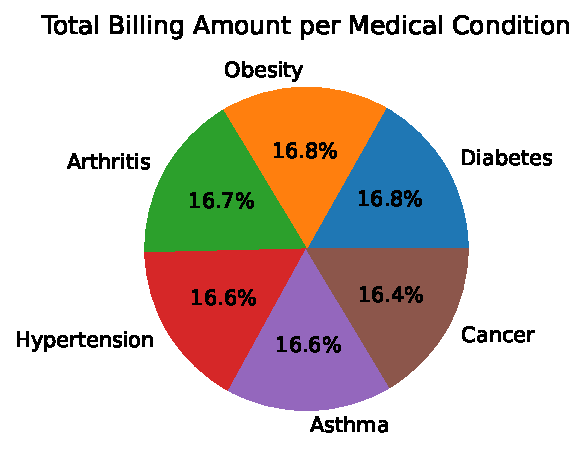
\includegraphics{index_files/figure-pdf/fig-margin-cap-output-1.pdf}

}

\caption{\label{fig-margin-cap}Additionally, the person with the highest
bill was Karen Kline. She was billed a total 104746.064748 by United
Healthcare in the span of}

\end{figure}%

\textbackslash{}

\begin{verbatim}
Name
kARen klInE    104746.064748
Name: Billing Amount, dtype: float64
\end{verbatim}

I decided to understand how diabetes was being treated and how it would
affect the cost. This shows that the number one insurance provider for
people with Diabetes was Medicare with 1730 patients total. Additionally
Medicare had the highest amount billed which could be to to the the fact
that they had more patients.

\begin{Shaded}
\begin{Highlighting}[]
\NormalTok{diabetes }\OperatorTok{=}\NormalTok{ df[df[}\StringTok{\textquotesingle{}Medical Condition\textquotesingle{}}\NormalTok{] }\OperatorTok{==} \StringTok{\textquotesingle{}Diabetes\textquotesingle{}}\NormalTok{]}
\NormalTok{df\_unique }\OperatorTok{=}\NormalTok{ diabetes.drop\_duplicates(subset}\OperatorTok{=}\StringTok{\textquotesingle{}Name\textquotesingle{}}\NormalTok{, keep}\OperatorTok{=}\StringTok{\textquotesingle{}first\textquotesingle{}}\NormalTok{)}
\NormalTok{insurance }\OperatorTok{=}\NormalTok{ df\_unique[}\StringTok{\textquotesingle{}Insurance Provider\textquotesingle{}}\NormalTok{].value\_counts()}
\BuiltInTok{print}\NormalTok{(insurance)}

\NormalTok{costly }\OperatorTok{=}\NormalTok{ df.groupby(df\_unique[}\StringTok{\textquotesingle{}Insurance Provider\textquotesingle{}}\NormalTok{])[}\StringTok{\textquotesingle{}Billing Amount\textquotesingle{}}\NormalTok{].}\BuiltInTok{sum}\NormalTok{().sort\_values(ascending}\OperatorTok{=}\VariableTok{False}\NormalTok{).head(}\DecValTok{5}\NormalTok{)}
\end{Highlighting}
\end{Shaded}

\begin{verbatim}
Insurance Provider
Medicare            1730
Blue Cross          1683
Cigna               1679
Aetna               1668
UnitedHealthcare    1624
Name: count, dtype: int64
\end{verbatim}

Lipitor was the drug most likely prescribed to someone with diabetes. A
reason for this is that people with diabetes are twice as likely to have
\href{https://www.cdc.gov/diabetes/diabetes-complications/diabetes-and-your-heart.html}{heart
disease} or a stroke compared to people without diabetes. Medications
such as Lipitor are effective at lowering low-density lipoprotein (LDL)
cholesterol lowering the chances of a stroke. However, penicilin was the
the medication that was billed the most.

\begin{Shaded}
\begin{Highlighting}[]
\NormalTok{medication }\OperatorTok{=}\NormalTok{ diabetes[}\StringTok{\textquotesingle{}Medication\textquotesingle{}}\NormalTok{].value\_counts()}
\BuiltInTok{print}\NormalTok{(medication)}

\NormalTok{plt.bar(medication.index, medication.values)}
\NormalTok{plt.xlabel(}\StringTok{\textquotesingle{}Medication\textquotesingle{}}\NormalTok{)}
\NormalTok{plt.ylabel(}\StringTok{\textquotesingle{}Frequency\textquotesingle{}}\NormalTok{)}
\NormalTok{plt.title(}\StringTok{\textquotesingle{}Frequency of Medications\textquotesingle{}}\NormalTok{)}
\NormalTok{plt.show()}
\end{Highlighting}
\end{Shaded}

\begin{verbatim}
Medication
Lipitor        1893
Penicillin     1881
Ibuprofen      1861
Aspirin        1858
Paracetamol    1811
Name: count, dtype: int64
\end{verbatim}

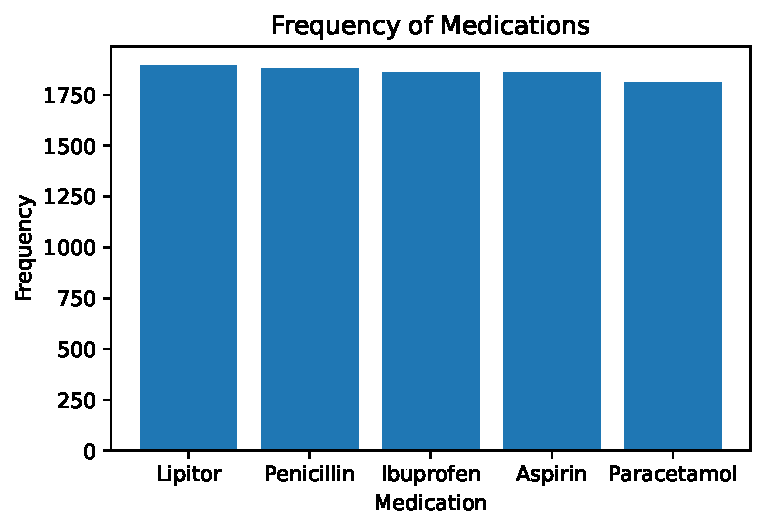
\includegraphics{index_files/figure-pdf/cell-6-output-2.pdf}

\begin{Shaded}
\begin{Highlighting}[]
\NormalTok{costmed }\OperatorTok{=}\NormalTok{ df.groupby(diabetes[}\StringTok{\textquotesingle{}Medication\textquotesingle{}}\NormalTok{])[}\StringTok{\textquotesingle{}Billing Amount\textquotesingle{}}\NormalTok{].}\BuiltInTok{sum}\NormalTok{().sort\_values(ascending}\OperatorTok{=}\VariableTok{False}\NormalTok{).head(}\DecValTok{5}\NormalTok{)}


\NormalTok{newdf }\OperatorTok{=}\NormalTok{ diabetes[[}\StringTok{\textquotesingle{}Medication\textquotesingle{}}\NormalTok{, }\StringTok{\textquotesingle{}Insurance Provider\textquotesingle{}}\NormalTok{, }\StringTok{\textquotesingle{}Billing Amount\textquotesingle{}}\NormalTok{]]}

\NormalTok{medication\_billing }\OperatorTok{=}\NormalTok{ newdf.groupby([}\StringTok{\textquotesingle{}Insurance Provider\textquotesingle{}}\NormalTok{, }\StringTok{\textquotesingle{}Medication\textquotesingle{}}\NormalTok{])[}\StringTok{\textquotesingle{}Billing Amount\textquotesingle{}}\NormalTok{].}\BuiltInTok{sum}\NormalTok{().sort\_values(ascending}\OperatorTok{=}\VariableTok{False}\NormalTok{).head(}\DecValTok{8}\NormalTok{).reset\_index()}
\BuiltInTok{print}\NormalTok{(medication\_billing)}
\end{Highlighting}
\end{Shaded}

\begin{verbatim}
  Insurance Provider   Medication  Billing Amount
0           Medicare      Aspirin    1.076458e+07
1              Cigna      Lipitor    1.039165e+07
2              Aetna  Paracetamol    1.014584e+07
3              Aetna   Penicillin    9.897654e+06
4              Cigna   Penicillin    9.862867e+06
5         Blue Cross    Ibuprofen    9.843164e+06
6         Blue Cross      Lipitor    9.768164e+06
7           Medicare  Paracetamol    9.748423e+06
\end{verbatim}

plot(1:10)

And then set the caption location in the code chunk like this:

```yaml \#\textbar{} label: fig-margin-cap \#\textbar{} fig-cap: ``This
is a caption in the margin.'' \#\textbar{} caption-location: margin



\end{document}
